\chapter{ROS}

\section{Concepts}
\url{https://wiki.ros.org/ROS/Concepts}
    \subsection{Filesystem level}
        \begin{itemize}
            \item packages
            \item meta packages
            \item package manifests
            \item repositories
            \item message/msg types
            \item service/srv types
        \end{itemize}
    \subsection{Computation graph level concepts}
        \begin{itemize}
            \item Node \url{}
            \item Master \url{}
            \item Parameter server \url{}
            \item messages \url{}
            \item topics \url{}
            \item services \url{}
            \item bags \url{}
        \end{itemize}
    \subsection{Names}
        bbc
        

\section{Setup}
    \subsection{TF}
        \url{https://wiki.ros.org/navigation/Tutorials/RobotSetup/TF}
        \begin{figure}
            \centering
            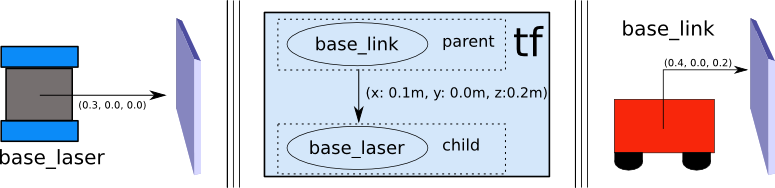
\includegraphics{\figspath ros/tf}
            \caption{}
            \label{fig:tf}
        \end{figure}
\section{Names}
    see \url{https://wiki.ros.org/Names}
    \begin{itemize}
        \item global
        \item relative
        \item private
        \item base
    \end{itemize}

\section{TF}
    A package responsible for managing and publishing coordinate frames and transformation between them.
    
    TF keeps all the frames in a directed tree called ''Transform tree''
    
    
    map is coming from GPS which is from world frame. base\_link is robots body and lidar\_link as well
    map → odom → base\_link → lidar\_link
    
    \paragraph{time\_stamped}
        Each transform is published with timestamp
        
\section{ROSPlan}
    The ROSPlan framework provides a collection of tools for AI Planning in a ROS system. ROSPlan has a variety of nodes which encapsulate plan, problem generation, and plan execution.
    \url{https://kcl-plan.github.io/ROSPlan/documentation/}
\section{Messages}
    \subsection{geometry\_msgs}
    \subsection{nav\_msgs}
        \paragraph{Odometry}
            has Pose of 7 dimensions (3 for position and 4 quaternions) and 6 as twist or velocity (3 linear velocity and 3 angular)
    \subsection{sensor\_msgs}
        \paragraph{LaserScan}
    \subsection{diagnostic\_msgs}
    \subsection{actionlib\_msgs}
\section{Topics}
    Is a communication channel to which nodes can publish messages or subscribe for messages

    \paragraph{Notes}
        They are ros runtime proccesses
        \begin{itemize}
            \item each topic can have as many publishers and subscribers that you need but the message types must be always the same
        \end{itemize}
\section{Node}
    Node a piece of runable code in ROS. It is either a c++/python code or a Gazebo plugin

    to list the running node:
    \begin{minted}{bash}
        rosnode list
    \end{minted}
\section{RQT Graph}
    Is a visual tool that shows nodes as boxes and topics as ovals and the direction of the edges show publisher and subscriber nodes
\section{RQT console}
    To visualize logs
\section{Bags}
\section{Frames}
     startes by world frame and then main robot's frame.
    
    Frames can have children. for example uav2/gps\_origin is the parent of uav2/fcu in which fcu is the the flight controller unit.
\section{Parameters}
    \url{https://wiki.ros.org/Parameter%20Server}
    \subsection{Parameter server}
\section{Services}
    request-response communication form. Such as calling gazebo/get\_model\_state and getting models location
\section{Action}
    \url{https://wiki.ros.org/actionlib}
    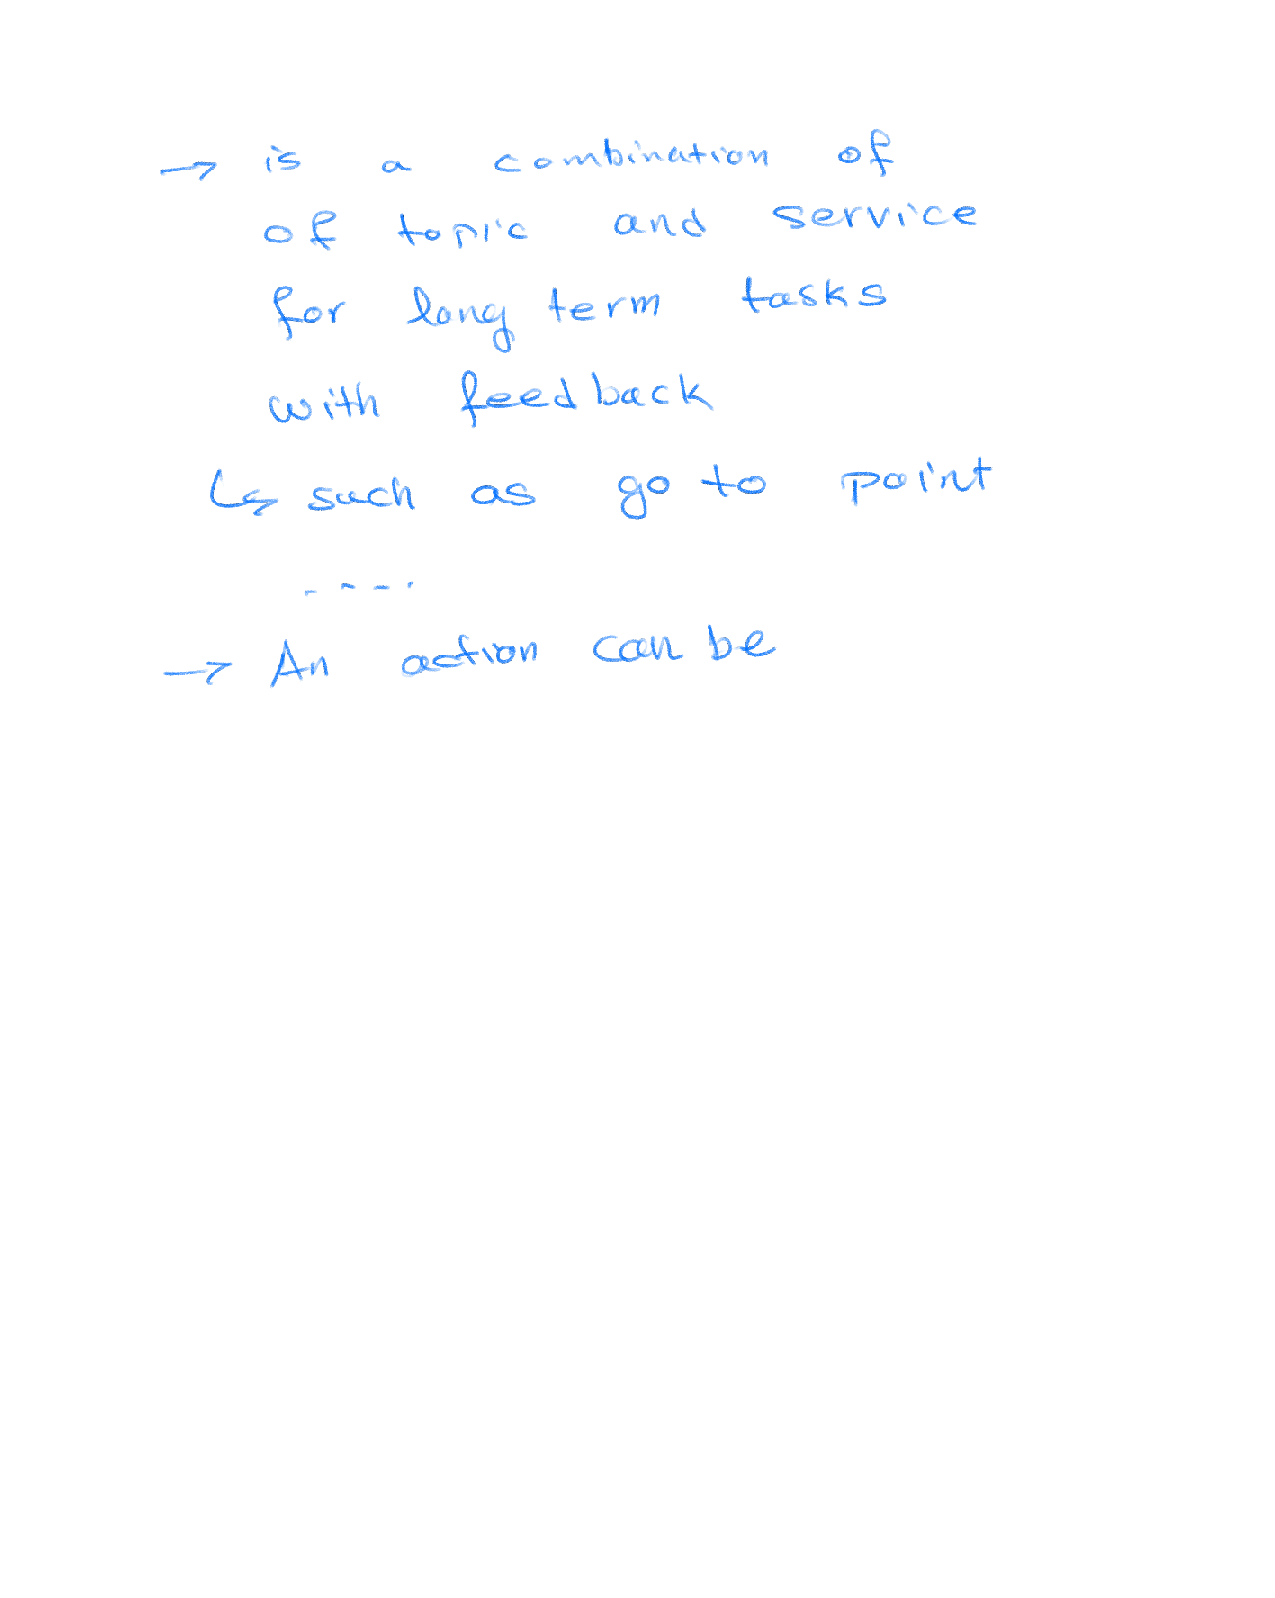
\includepdf[pages=-]{\figspath ros/action.pdf}
    \subsection{Goal}

Is a combination of services and topics for a longterm mission with feedback and result and it could be terminated in the middle.
    \paragraph{components}
        \subparagraph{Action client}
            Within application client
        \subparagraph{Action server}
            Within application server
    
    \paragraph{Messages}
        \subparagraph{Goal}
        \subparagraph{Feedback}
        \subparagraph{Result}

\section{Navigation}
    \url{https://wiki.ros.org/navigation?distro=noetic}

\section{Planning}
\section{rviz}
    For visualizing data from sensors
\section{MAVROS}
\section{MAVLINK}
\section{QGroundControl}
\section{Flight controller}
    It is the hardware board and it usually contains
    \begin{itemize}
        \item IMU
        \item Barometer (for height)
        \item GNSS
        \item Microcontroller/cpu
        \item I/O ports
    \end{itemize}

    examples:
    \begin{itemize}
        \item Pixhawk
        \item Cubeorange
        \item Holybro
    \end{itemize}

\section{Autopilot}
    \subsection{PX4}
        \subsection{PXmini}
    \subsection{Ardupilot}